\begin{figure*}[htbp]
    \centering
    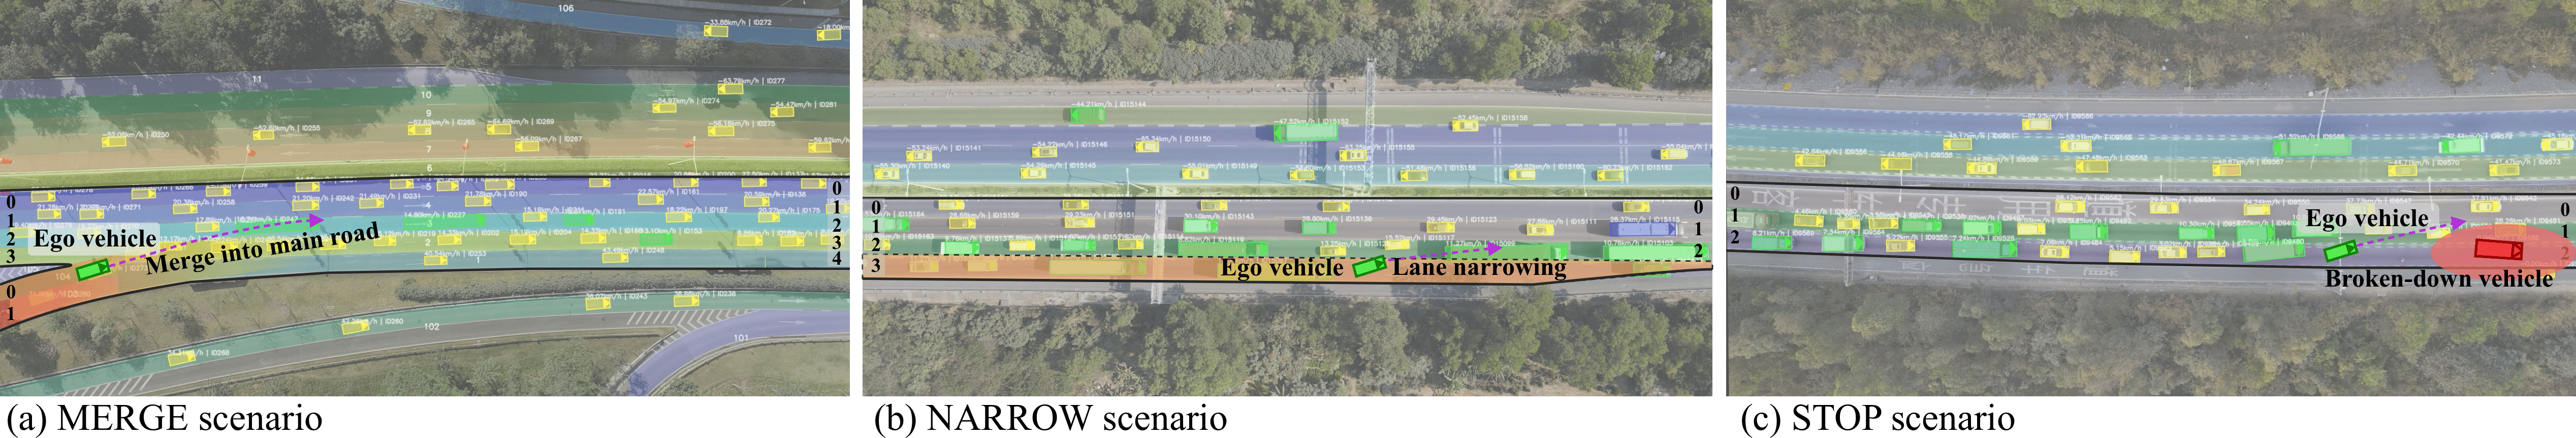
\includegraphics[width=\textwidth]{fig/sim.png}
    \caption{Three scenarios in the simulation environment: (a) MERGE: vehicle merging into the main lane from the ramp, (b) NARROW: vehicle navigating a narrowing right lane, (c) STOP: vehicle bypassing a broken-down vehicle.}
    \label{fig:sim}
\end{figure*}
\begin{figure*}[!htbp]
    \centering
    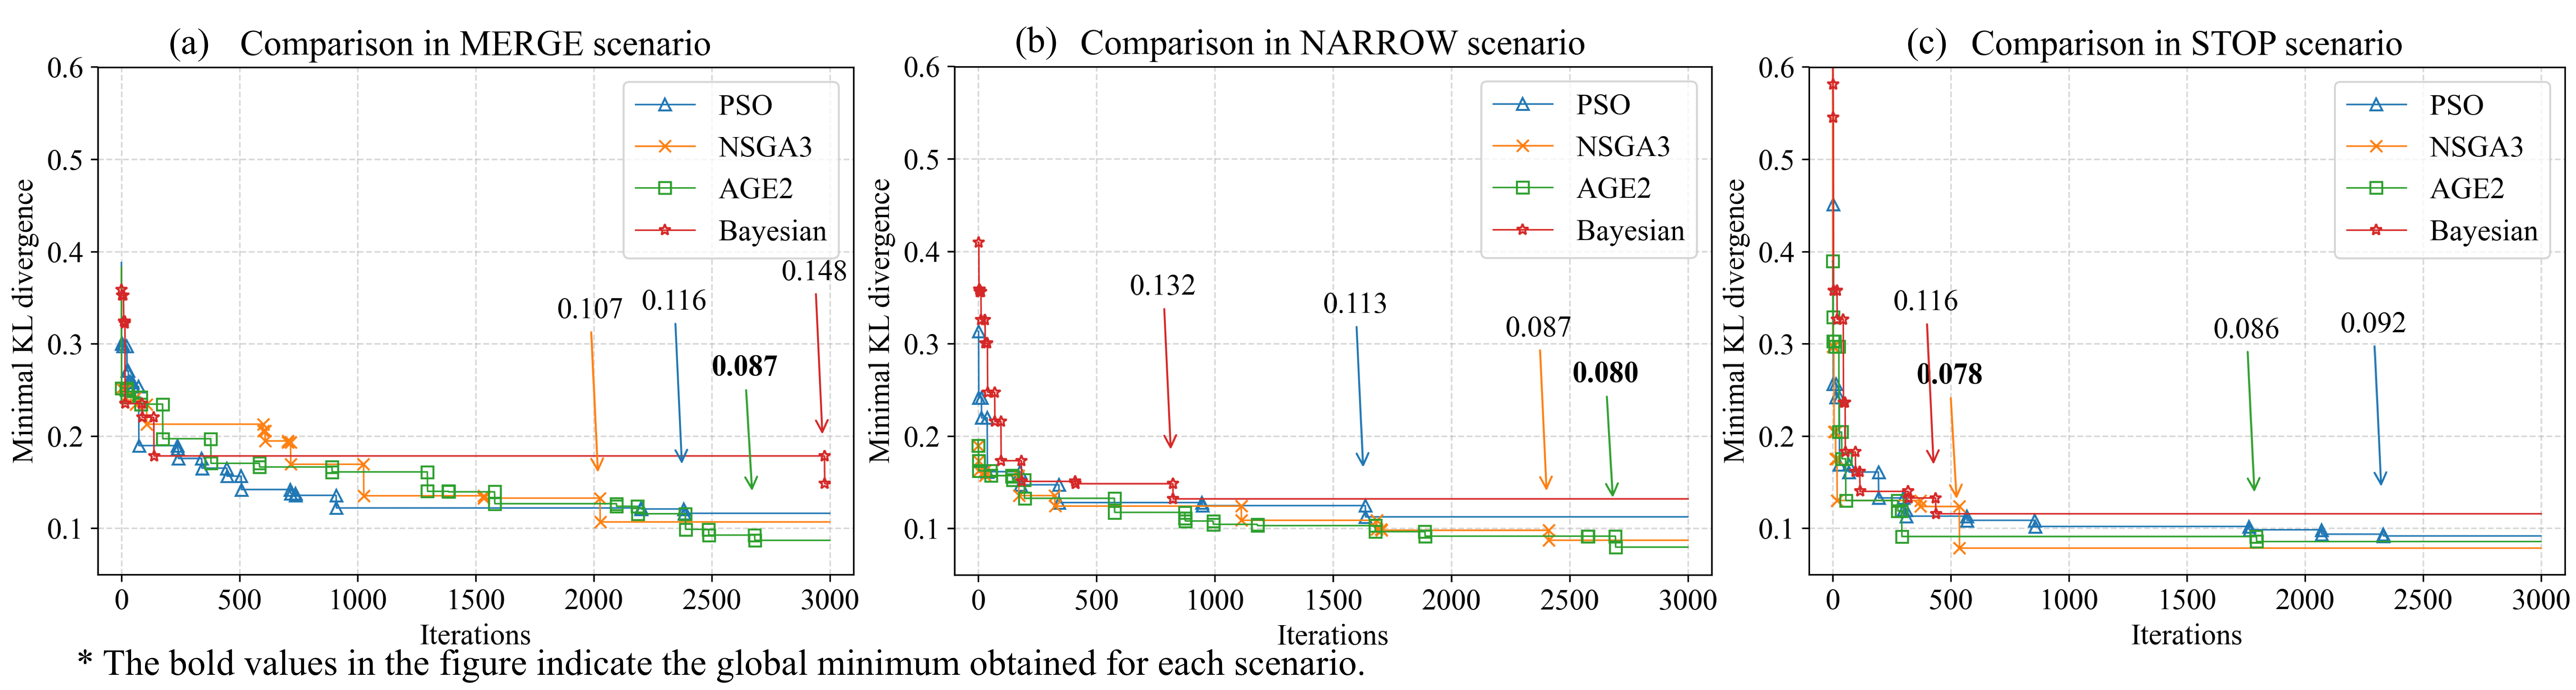
\includegraphics[width=\textwidth]{fig/env_iter.png}
    \caption{
        Convergence comparison of optimization objective in (a) MERGE scenario, (b) NARROW scenario, (c) STOP scenario. 
    }
    \label{fig:env_iter}
\end{figure*}

\begin{figure*}[!htbp]
    \centering
    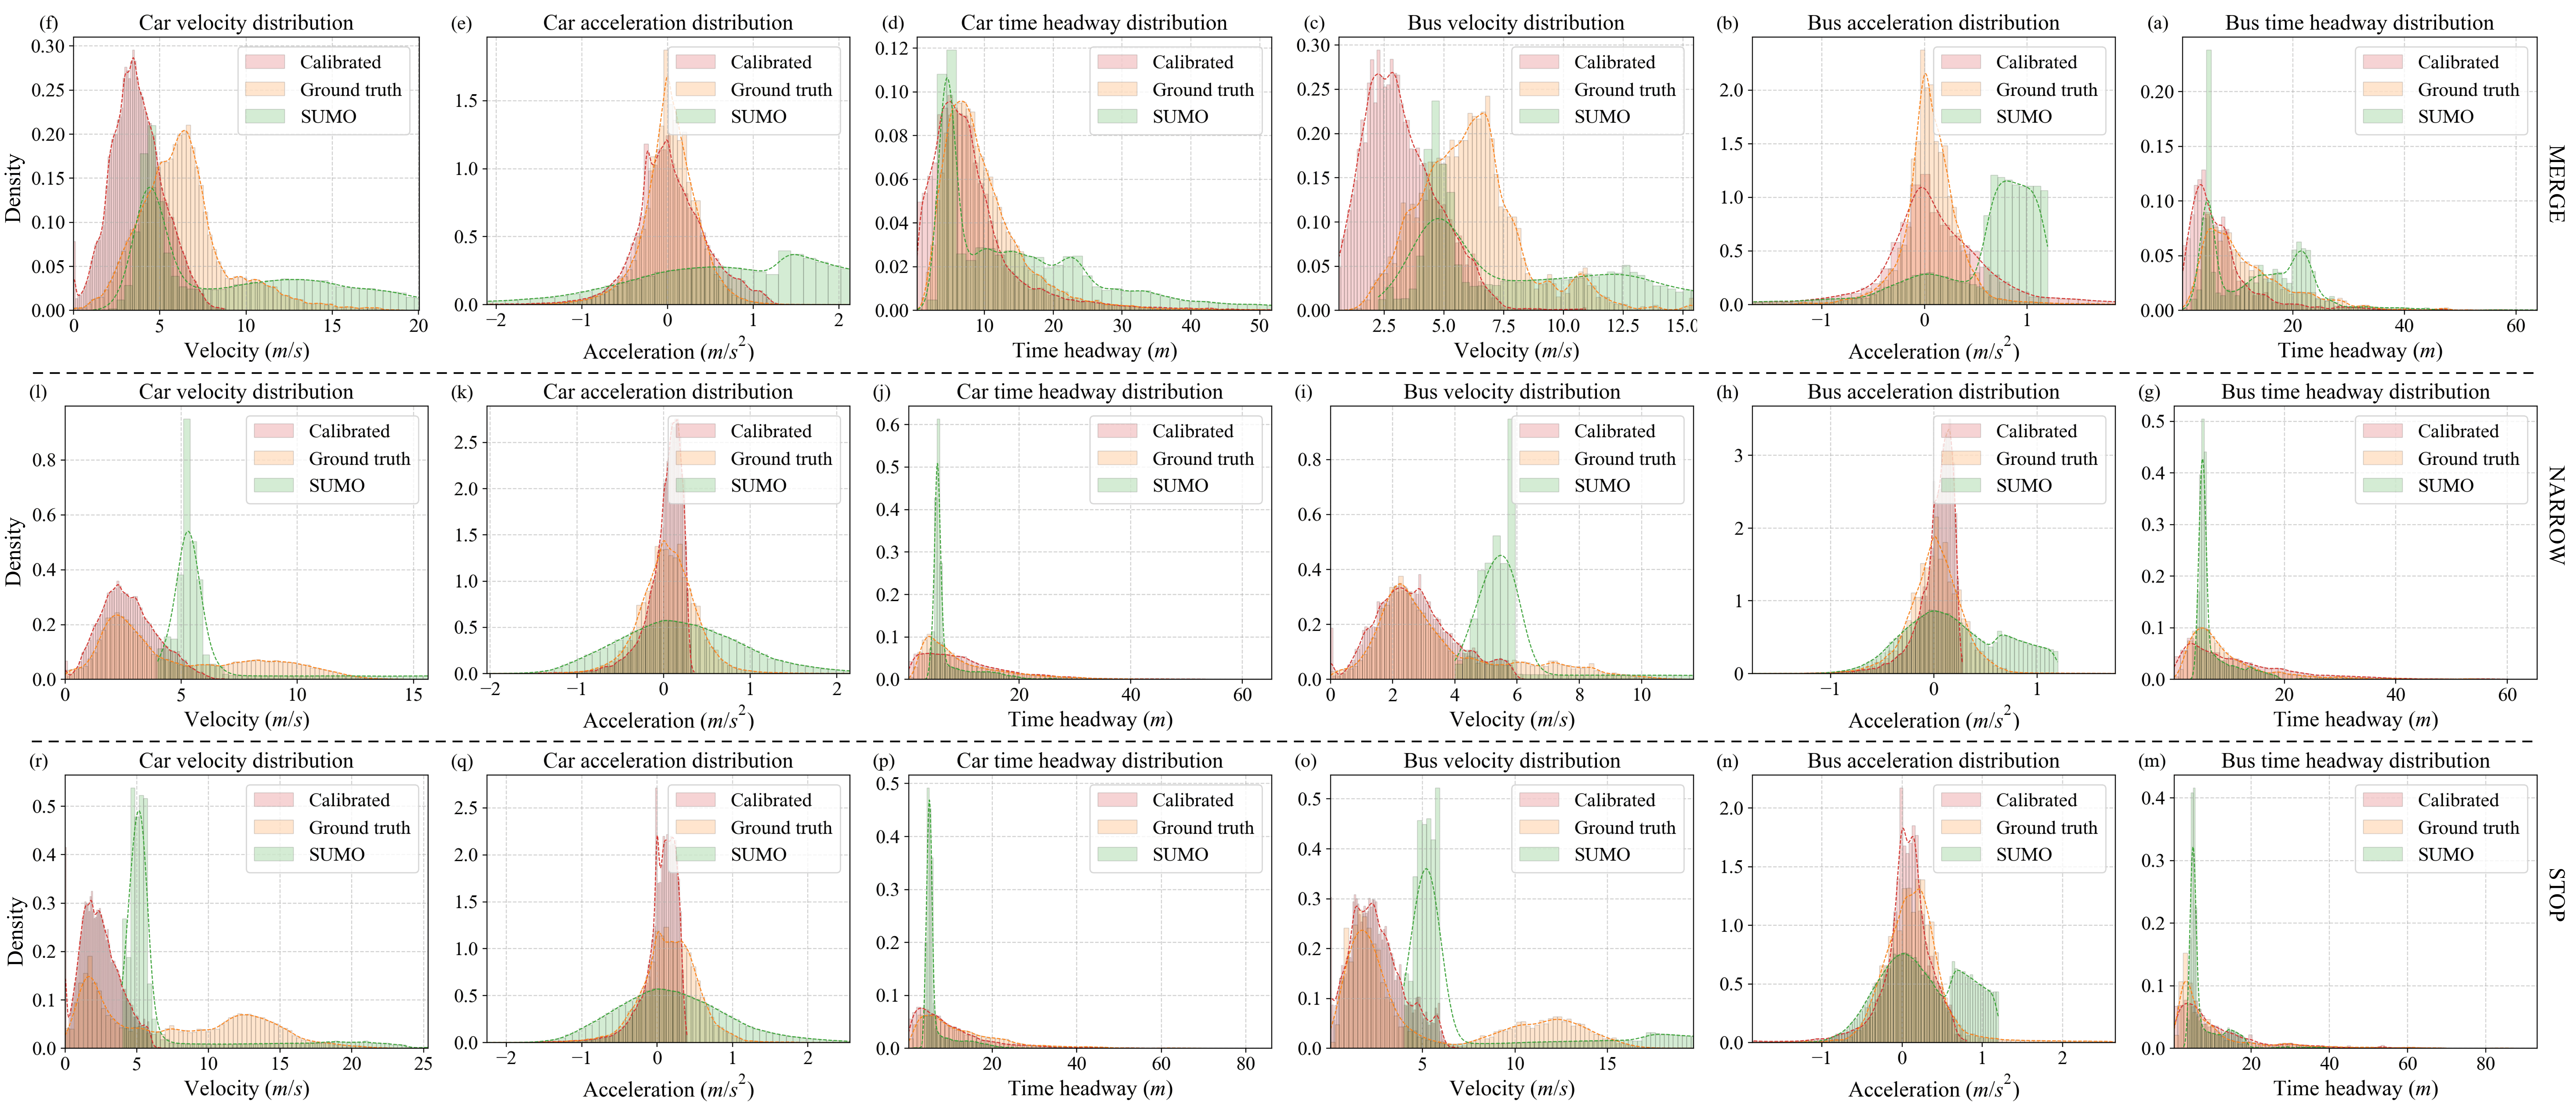
\includegraphics[width=\textwidth]{fig/env_dis.png}
    \caption{Comparison of calibration results for velocity, acceleration, and time headway distributions across three scenarios for cars and buses}
    \label{fig:env_distri}
\end{figure*}


\section{Experiments and Results}
\label{sec:experiments}
% I. Broad Context and Significance (Setting the Stage):
% A Opening Hook
This section details the experimental evaluation conducted to validate the performance of our proposed algorithm within realistic simulated traffic scenarios. We trained and evaluated our algorithm against seven baselines, followed by a comprehensive analysis of the experimental results, including an ablation study. The subsequent subsections elaborate on the experimental setup, traffic scenario generation, training procedures, and results analysis.

\subsection{Simulation Environment}
Adversarial congestion scenarios, including mandatory lane changes during merges, accidents, and lane narrowing, pose critical challenges to highway automation. These scenarios are major contributors to autonomous driving system failures \cite{naturecrash, nordhoff2024conceptual}. To evaluate our method's performance under such conditions, we utilized the AD4CHE dataset \cite{AD4CHE}, which focuses on congestion on Chinese highways and urban highways.

We selected three representative scenarios from AD4CHE's aerial data (5.12 hours total): (a) Merge scenario (files 1-8), where the ego vehicle merges from a two-lane road onto a four-lane highway, requiring conflict resolution in the merging zone; (b) Narrow scenario (files 18-23), where the ego vehicle must change lanes leftward before a road narrowing; and (c) Stop scenario (files 15-16), where the ego vehicle navigates around a broken-down vehicle in slow-moving traffic.  These scenarios are illustrated in Fig. \ref{fig:sim}.

\subsection{Trustworthy Traffic Scenario Generation}

We utilize SUMO\cite{SUMO2018} (Simulation of Urban MObility) to create the simulation environment. Four optimization algorithms—PSO\cite{pso}, Bayesian\cite{bayesian}, NSGA3\cite{NSGA3}, and AGE2\cite{AGE2}—are employed to minimize the KL divergence between the aggregated real-world and simulated data for acceleration, velocity, and time headway. Each algorithm iterates 3000 times (population-based and evolutionary algorithms use 100 populations$\times$30 iterations to ensure fair results.)

The calibrated aggregated traffic flow metrics include acceleration, velocity, and time headway distributions for both car and bus vehicle types. These calibration results are compared against both the real-world dataset and the original SUMO-generated metrics. The calibration process was done in a workstation equipped with 2$\times$AMD 5995WX CPU (128 cores total) and 256GB of RAM, required approximately 24 hours to complete 3000 iterations across three scenarios for four algorithms.

Fig. \ref{fig:env_iter} shows the convergence comparison of the optimization objective in the three scenarios. The results show that all four optimization algorithms can reduce the error to a satisfactory level (mean KL divergence around 0.1). Single-objective algorithms (PSO, Bayesian) typically converge to the minimum value more quickly, while multi-objective algorithms (NSGA3, AGE2) ultimately achieve smaller values within a limited number of iterations. 

Fig. \ref{fig:env_distri} presents the distributions of multiple calibrated traffic flow aggregation metrics, compared with both the real dataset and uncalibrated original SUMO-generated metrics. The results demonstrate that, except for a few scenarios shown in Fig. \ref{fig:env_distri} (c) and (f), the calibrated metric distributions generally align with the true dataset in terms of central tendency, while the original SUMO-generated distributions typically exhibit wider dispersion. The time headway distributions in both real and calibrated data reveal a characteristic skewed pattern with peaks at smaller time intervals, indicating the presence of aggressive driving behaviors in the dataset. The original SUMO distributions shows significant deviations at larger time headways ($\ge$\SI{10}{\meter}), particularly underestimating the frequency of large time headways in complex scenarios such as MERGE and NARROW.
Regarding acceleration, the calibrated distributions show a more pronounced peak near zero acceleration, closely matching the ground truth distribution, while the SUMO distribution exhibits a shifted peak.  In the STOP scenario, SUMO severely underestimates the frequency of negative accelerations, whereas the calibrated model more accurately reflects actual braking behavior. Finally, the calibrated speed distributions effectively capture the bimodal characteristics (a high-frequency region and a more dispersed long-tail distribution), significantly outperforming SUMO. This improvement is particularly evident in the MERGE and STOP scenarios for cars, where SUMO notably overestimates speeds in the mid-range (e.g., \SIrange{5}{10}{\metre\per\second}) and underestimates the long-tail low-speed region. The calibrated model demonstrably corrects these deficiencies.





\subsection{Agent Training and Evaluation Setup}
To ensure experimental reproducibility, all agents were trained across five random seeds, each for 1000 episodes. Each episode was limited to 3000 time steps. Both training and evaluation were performed in trustworthy traffic scenarios, as described earlier in this paper. 
The experiments were conducted on a workstation equipped with dual NVIDIA RTX 3090 GPUs, an AMD Ryzen 9950X CPU, and 64 GB of RAM. The training process took approximately 12 hours. The following sections provide detailed information on the agent configuration.

\begin{figure}[H]
    \centering
    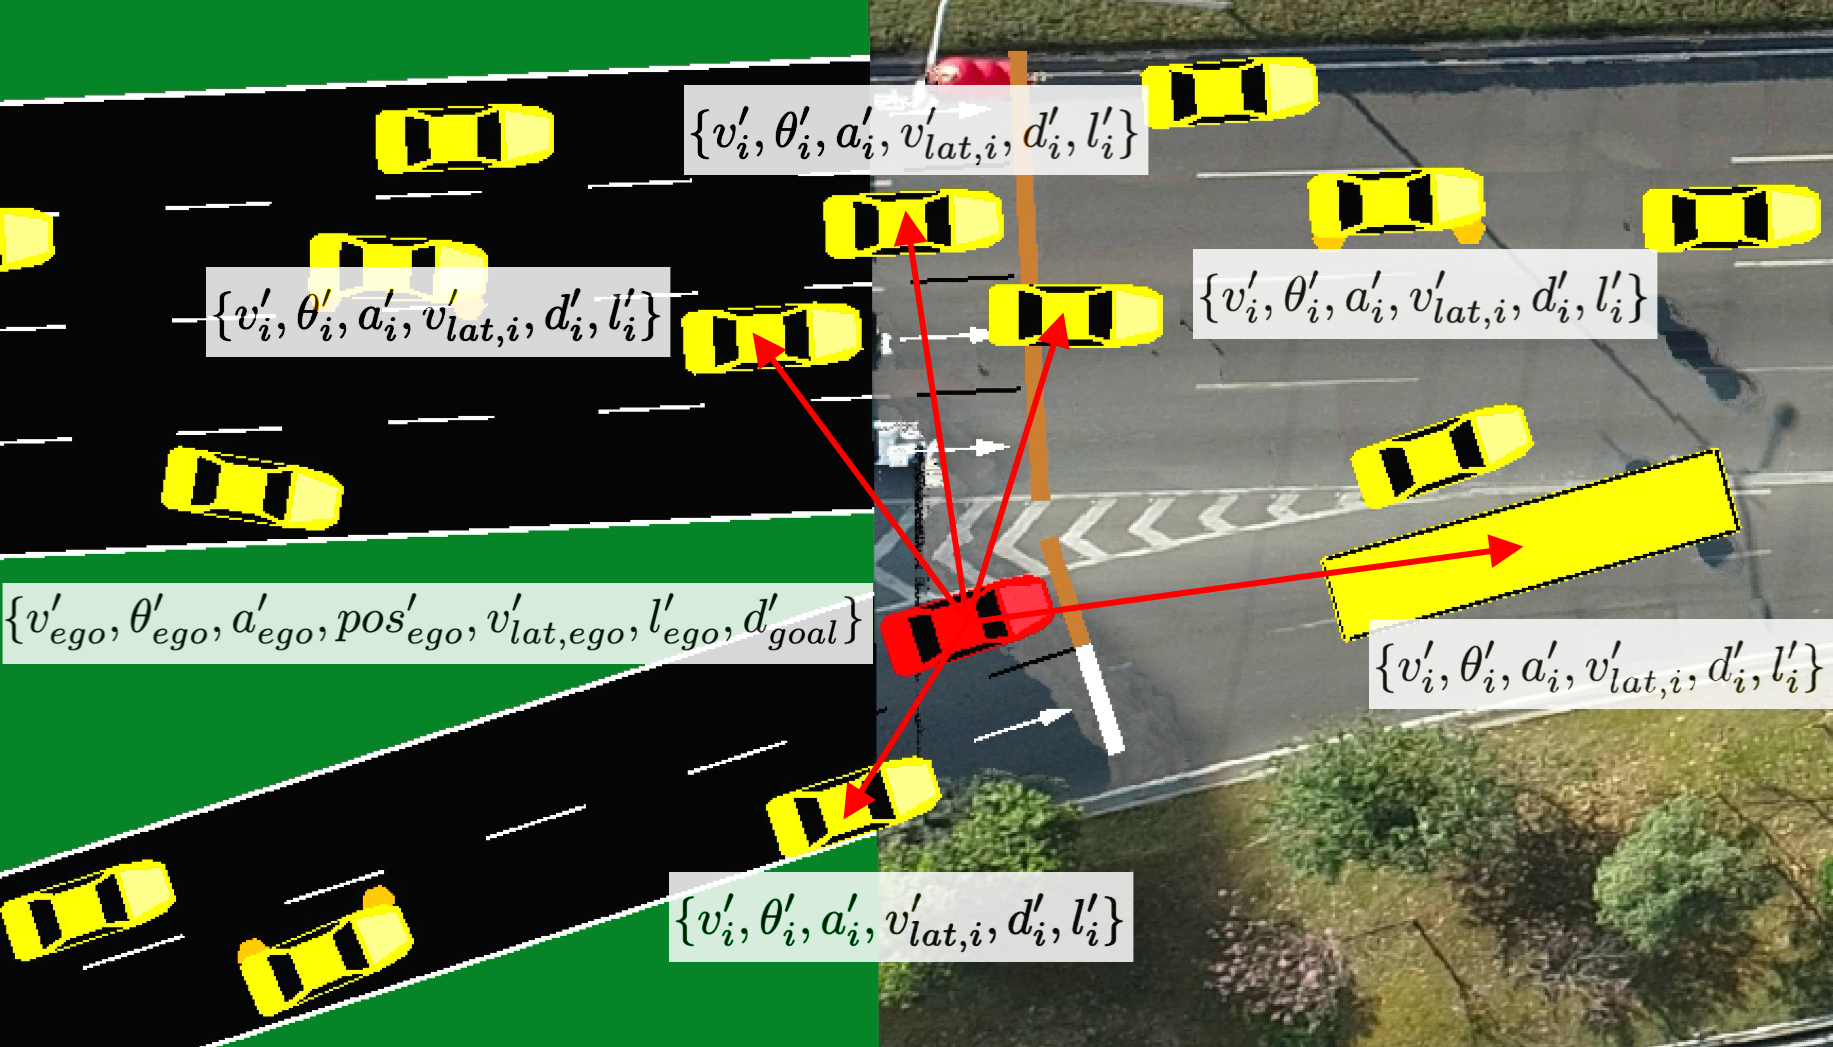
\includegraphics[width=0.49\textwidth]{fig/sim_set_up.png}
    \caption{Observation space for ego agent}
    \label{fig:sim_set_up} 
\end{figure}




\textbf{Observation Space:}
The observation space $\mathbf{o}_{t}$ is updated at \SI{10}{\hertz} and provides the agent's perception of its surroundings. It is formed by concatenating the observation vectors of the five nearest vehicles within a \SI{100}{\meter} detection range, together with the ego vehicle's own state as shown in Fig. \ref{fig:sim_set_up}. The observation space is defined as:
\begin{equation}
    \mathbf{o}_{t} = [\mathbf{o}_{\text{veh},i}]_{i=1, \ldots, 5} \oplus \mathbf{o}_{\text{ego}}.
\end{equation}

For each of the five nearest vehicles ($i = 1, 2, \ldots, 5$), the observation vector is a 6-dimensional set of normalized parameters:
\begin{equation}
    \mathbf{o}_{\text{veh},i} = \{v'_{\text{i}}, \theta'_{\text{i}}, a'_{\text{i}}, v'_{\text{lat},i}, d'_{\text{i}}, l'_{\text{i}}\},
\end{equation}
where $v'_{\text{i}}$, $\theta'_{\text{i}}$, $a'_{\text{i}}$, $v'_{\text{lat},i}$, $d'_{\text{i}}$, and $l'_{\text{i}}$ respectively represent the $i$-th vehicle's normalized speed, angle, acceleration, lateral speed, distance, and length.

The ego vehicle's observation vector consists of seven dimensions:
\begin{equation}
    \mathbf{o}_{\text{ego}} = \{v'_{\text{ego}}, \theta'_{\text{ego}}, a'_{\text{ego}}, pos'_{\text{ego}}, v'_{\text{lat,ego}}, l'_{\text{ego}}, d'_{\text{goal}}\},
\end{equation}
incorporating the ego vehicle's normalized speed, angle, acceleration, lane position, lateral speed, length, and distance to goal.

Table~\ref{tab:obs} summarizes each variable in the observation space:

\begin{table}[!ht]
    \centering
    \caption{Observation variables and their normalization.}
    \label{tab:obs}
    \begin{tabularx}{\columnwidth}{cX} % 使用 cX,第一列居中,第二列 X 列默认居中
    \toprule
    \textbf{Symbol} & \textbf{Description and Normalization} \\
    \midrule
    $v'_{\text{i}}, v'_{\text{ego}}$           & Vehicle speed, normalized by $v_{\text{max}}$ \\
    $\theta'_{\text{i}}, \theta'_{\text{ego}}$ & Vehicle angle, normalized by $\theta_{\text{max}}$ \\
    $a'_{\text{i}}, a'_{\text{ego}}$           & Vehicle acceleration, normalized by $a_{\text{max}}$ \\
    $v'_{\text{lat},i}, v'_{\text{lat,ego}}$   & Lateral speed, normalized by $v_{\text{lat,max}}$ \\
    $d'_{\text{i}}$                     & Distance to the $i$-th vehicle, normalized by $d_{\text{detect}}$ \\
    $l'_{\text{i}}, l'_{\text{ego}}$           & Vehicle length, normalized by $l_{\text{norm}}$ \\
    $pos'_{\text{ego}}$                 & Ego lane position, normalized by $d_{lane}$ \\
    $d'_{\text{goal}}$                  & Distance to goal, normalized by $d_{goal,init}$  \\
    \bottomrule
    \end{tabularx}
\end{table}

\textbf{Action Space:}
The action space $\mathbf{a}_t$ is a two-dimensional vector:
\begin{equation}
    \mathbf{a}_t = \{a_t, \delta_t\},
\end{equation}
where $a_t$ represents the acceleration and $\delta_t$ the lateral movement. Both components are continuous values within the range $[-1, 1]$. When interacting with the simulator, the acceleration $a_t$ is scaled by $a_{\text{max}}$, while $\delta_t$ remains unchanged as defined by the SUMO interface.


% =========debug=========
\textbf{Reward Function:}
The reward $\mathrm{R}$ is defined as Eq. \ref{eq:reward}:
\begin{equation}
    \label{eq:reward}
    \mathrm{R} = \alpha \cdot \frac{v_{\text{ego}}}{v_{\text{max}}}
          - \beta \cdot \bigl( \mathrm{C}_{\text{collision}} + \mathrm{C}_{\text{TTC}} + \mathrm{C}_{\text{overtime}} \bigr)
          + \gamma \cdot \mathrm{P}_{\text{nav}},
\end{equation}
where $\mathrm{C}_{\text{collision}} = \bigl(\mathrm{C}_{\text{base}} + v_{\text{col}}\bigr)$ if a collision occurs and $0$ otherwise.
$\mathrm{C}_{\text{TTC}}$ is defined as $\max\!\bigl(0, \,\text{TTC}_{\min} - \text{TTC}_{\text{ego}}\bigr)/\text{TTC}_{\min}$.
Meanwhile, $\mathrm{C}_{\text{overtime}} = \mathrm{C}_{\text{base}}\,(1 - \mathrm{P}_{\text{nav}})$ if the episode exceeds the time limit, and $0$ otherwise.
We measure progress as $\mathrm{P}_{\text{nav}} = 1$ if $d_{\text{goal}} < \SI{30}{\meter}$, or $1 - d_{\text{goal}} / d_{\text{goal,init}}$ otherwise.

The weighting parameters $\alpha$, $\beta$, and $\gamma$ are set to $1$, $1$, and $0.1$, respectively, based on a large-scale hyperparameter search.
The base collision cost $\mathrm{C}_{\text{base}}$ is $10$, and the minimum Time-To-Collision threshold $\text{TTC}_{\min}$ is \SI{3}{\second}.
Here, $v_{\text{ego}}$ is the ego vehicle's mean speed, $v_{\text{max}}$ its maximum speed, and $v_{\text{col}}$ the ego vehicle's speed upon collision.
The term $\text{TTC}_{\text{ego}}$ is the minimum Time-To-Collision with other vehicles during the episode, $d_{\text{goal}}$ is the distance to the goal when terminated, and $d_{\text{goal,init}}$ is the initial distance to the goal.


% ========================





\begin{figure*}[!htbp]
    \centering
    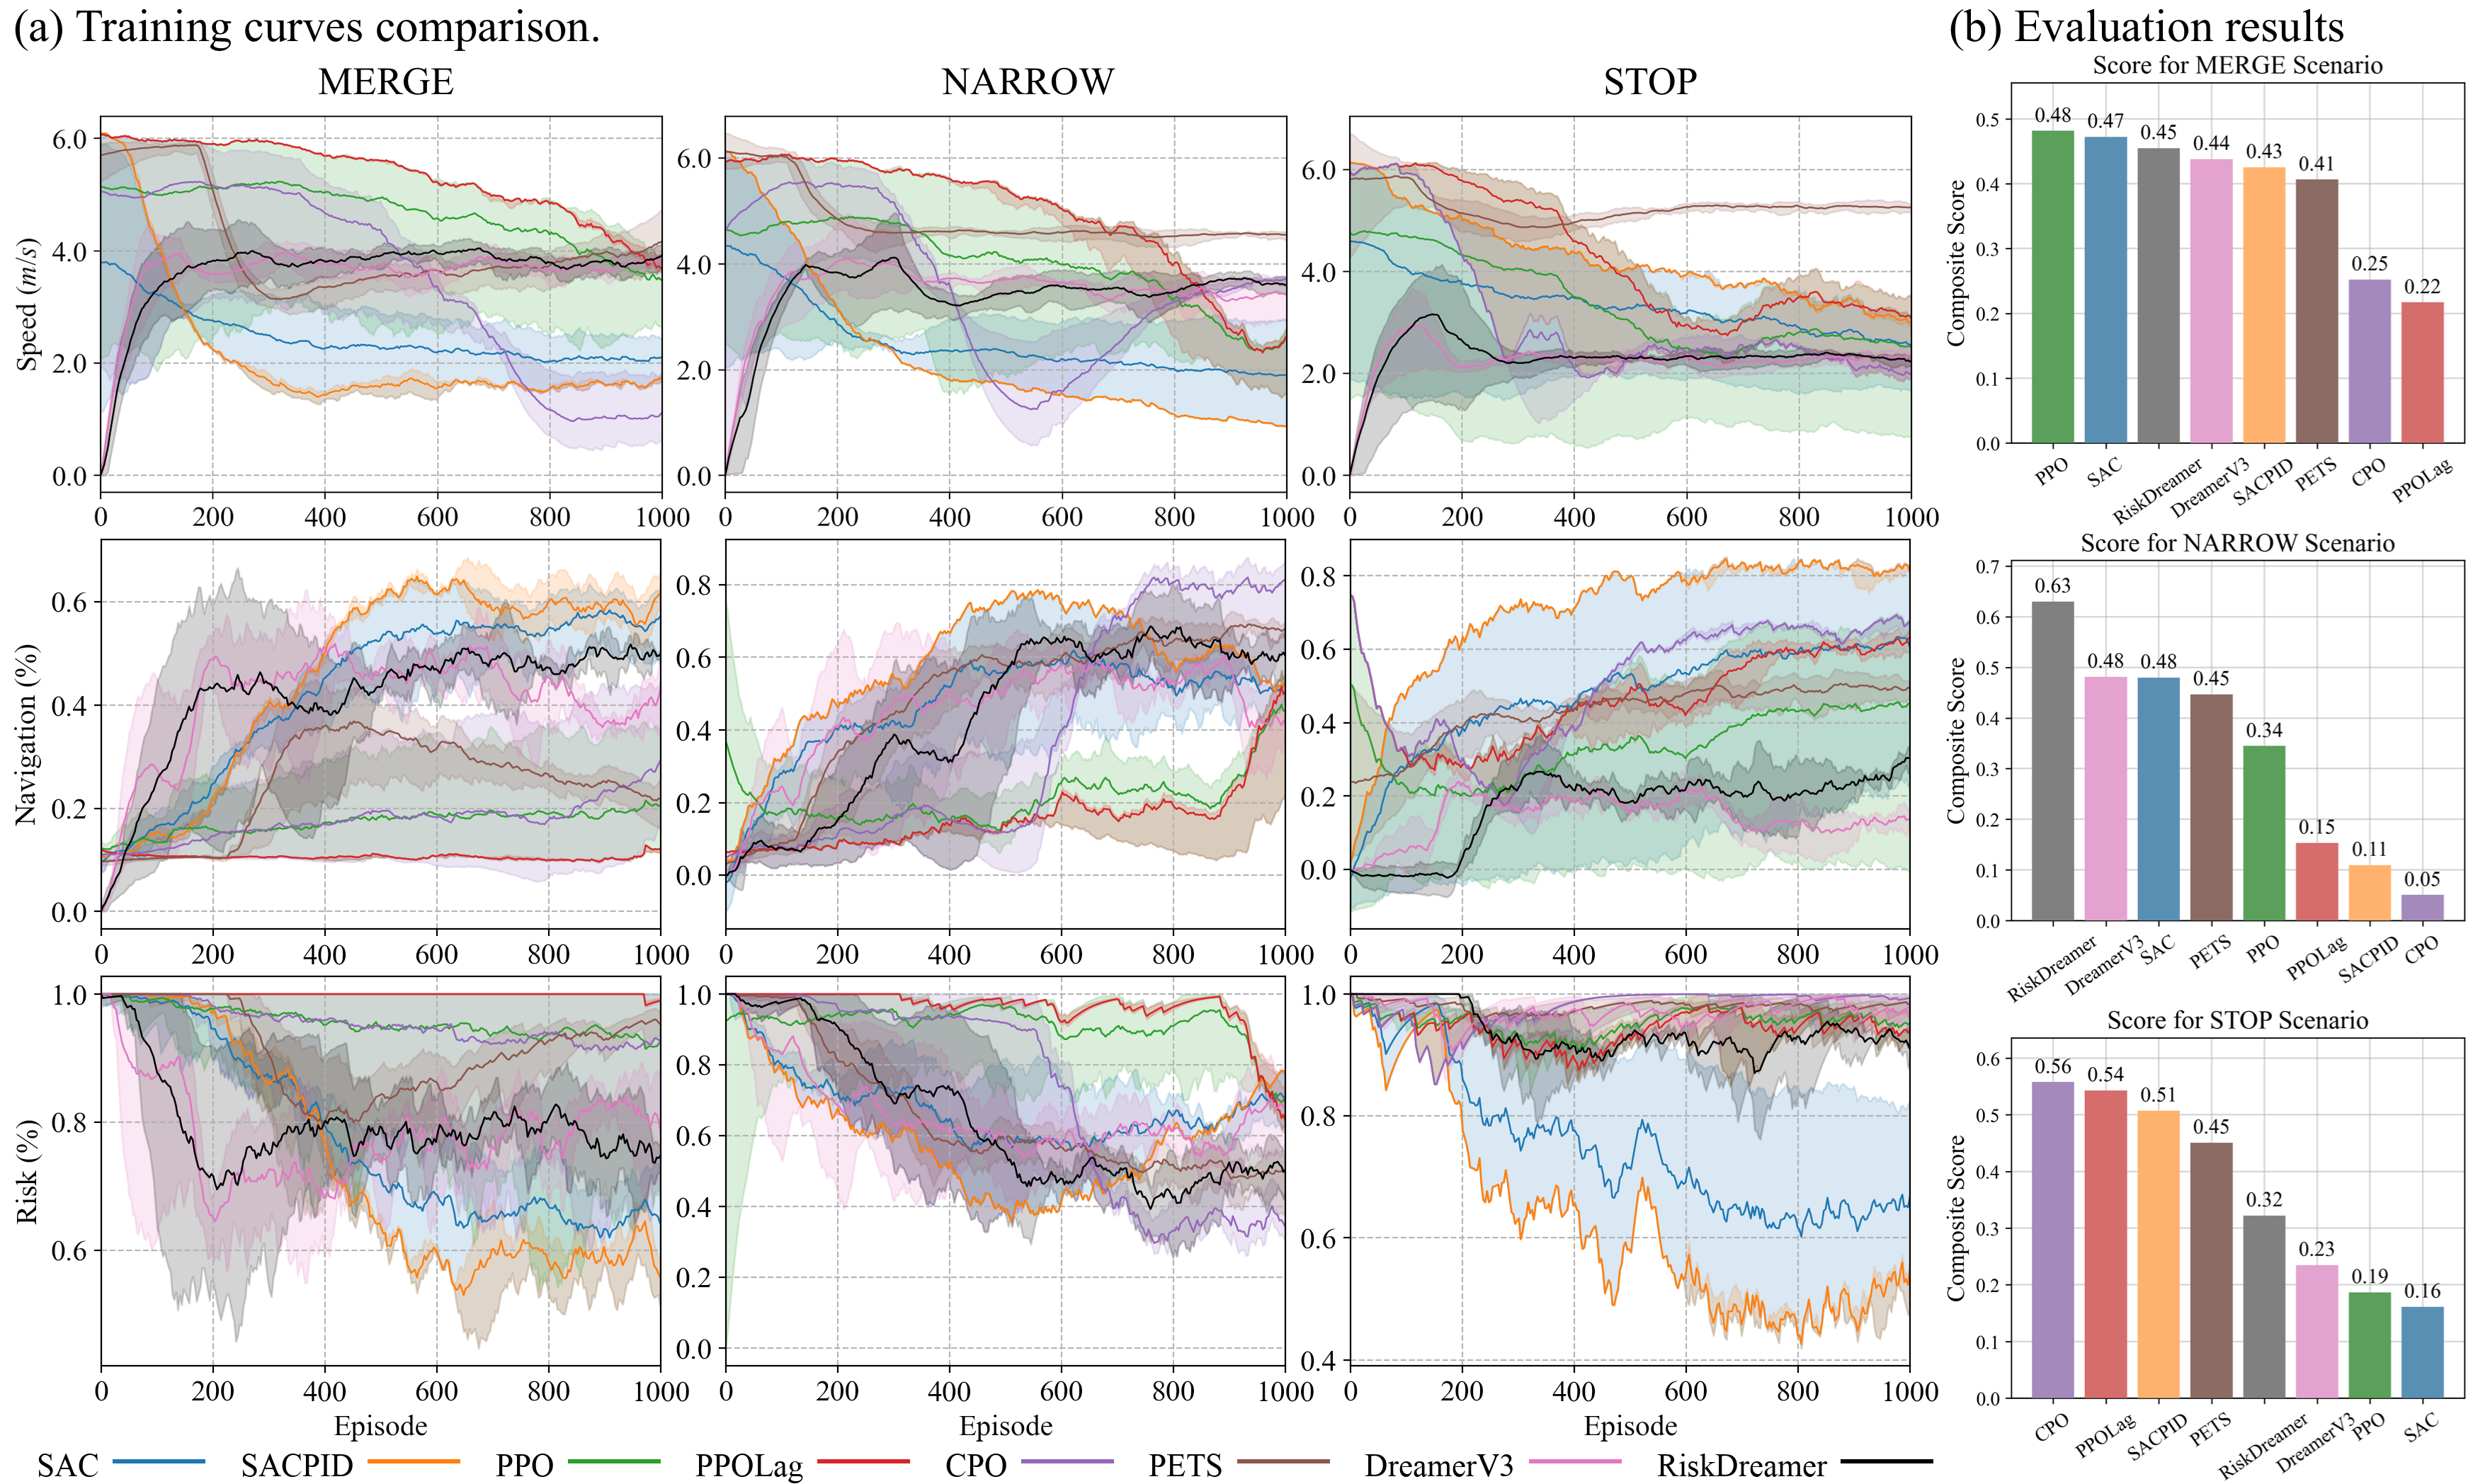
\includegraphics[width=\textwidth]{fig/train_curve.png}
    \caption{Results of different algorithm in the three scenarios. (a) Training curves comparison. (b) Evaluation results}
    \label{fig:train_curve}
\end{figure*}


\begin{figure*}[!htbp]
    \centering
    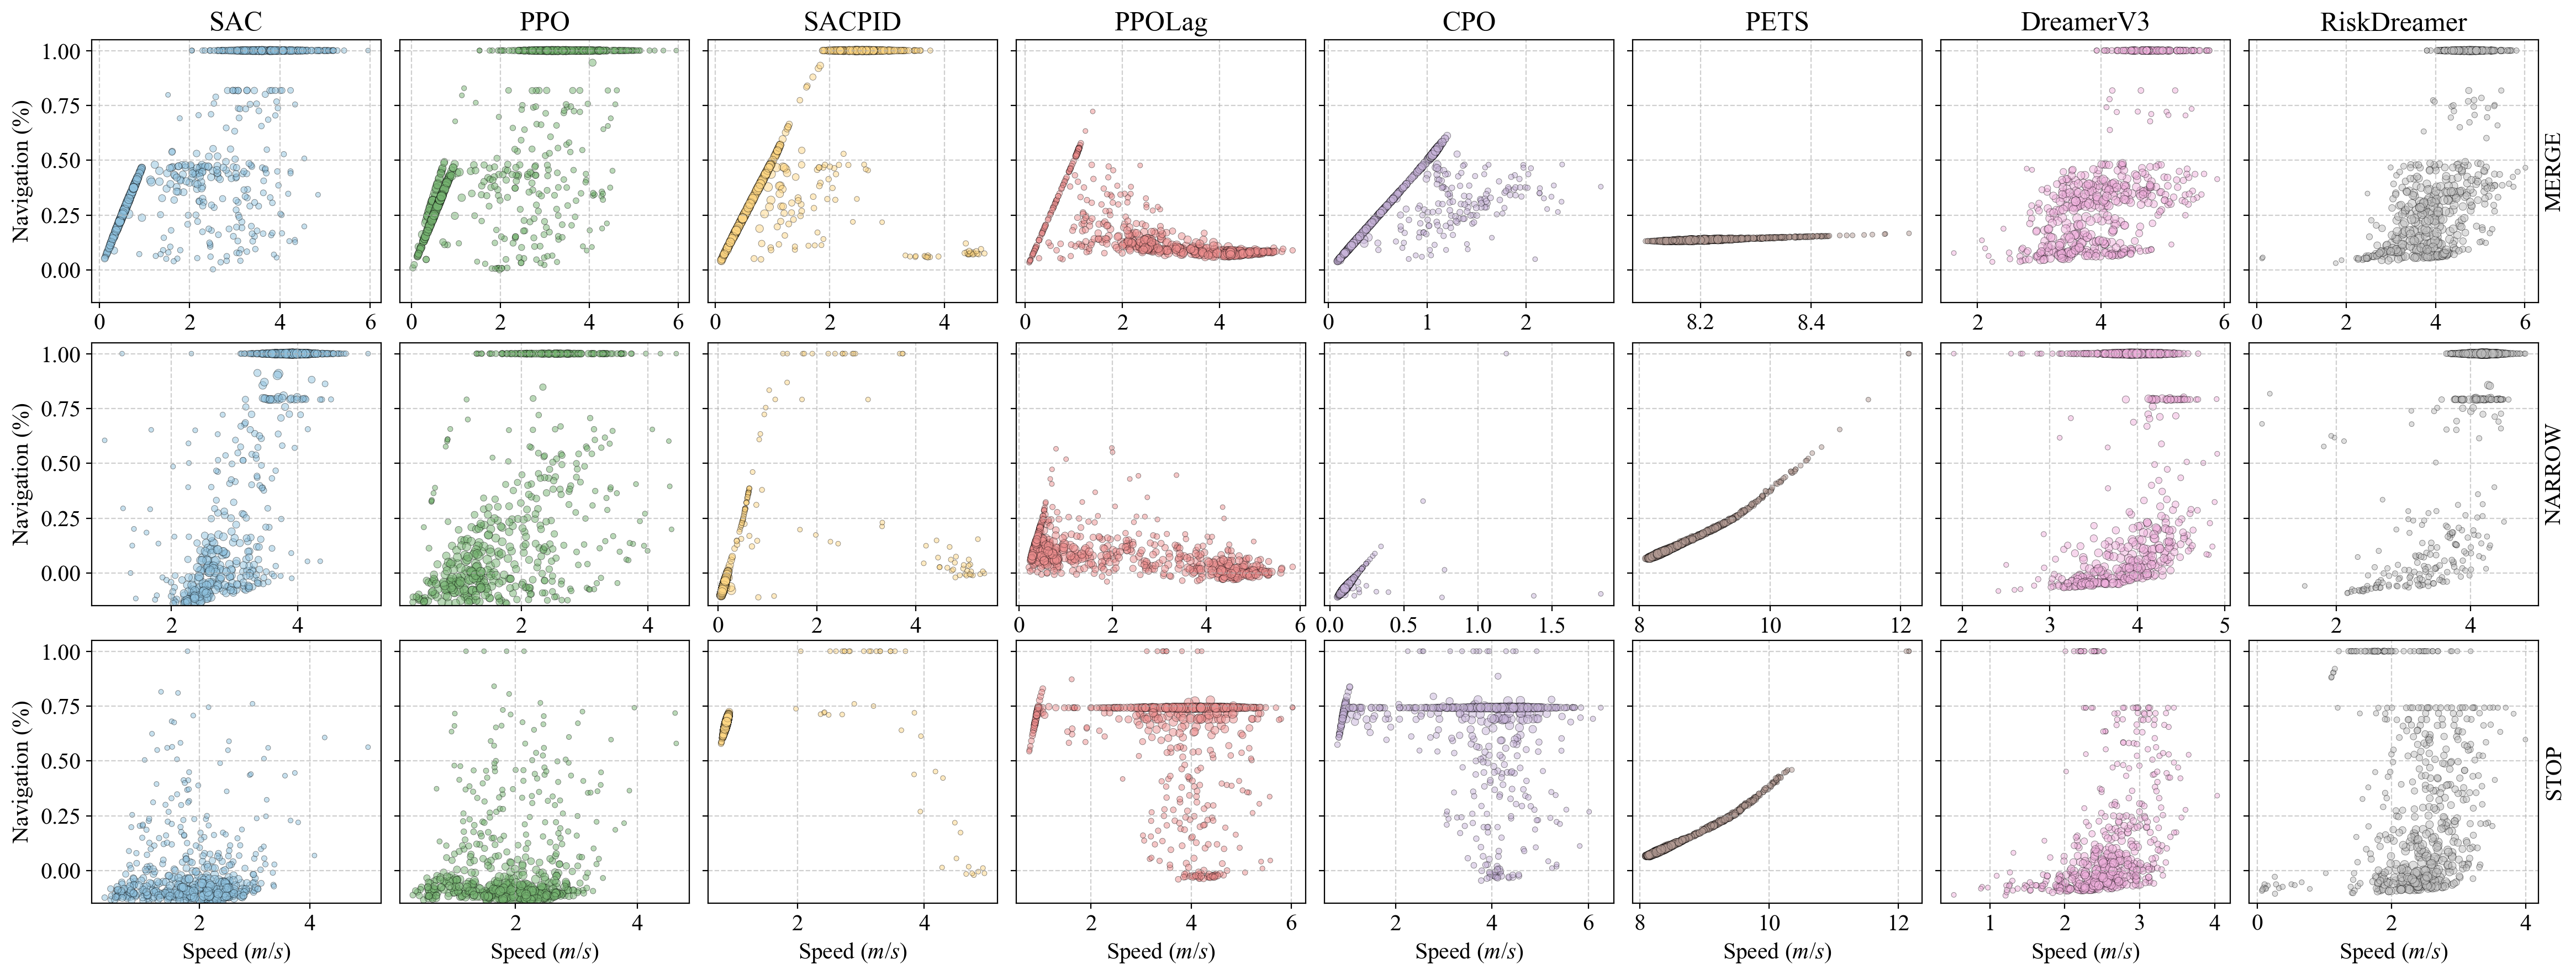
\includegraphics[width=\textwidth]{fig/algo_scatter_compare.png}
    \caption{Evaluation pattern of agent performance: Speed vs. Navigation. Bigger points indicate denser data point distributions.}
    \label{fig:eval}
\end{figure*}


\begin{table*}[tbp]
    \centering
    \caption{Performance comparison of different methods in multiple scenarios.}
    \label{table:comparison}
    \centering
    \setlength{\tabcolsep}{5pt}
    \begin{tabular}{p{1.4cm}m{1.6cm}p{0.78cm}p{0.78cm}p{0.78cm}p{0.78cm}p{0.78cm}p{0.78cm}p{0.78cm}p{0.78cm}p{0.78cm}p{0.78cm}p{0.78cm}p{0.78cm}}
        \toprule
        \textbf{Method} & \textbf{Metric} & \multicolumn{4}{c}{\textbf{MERGE Scenario}} & \multicolumn{4}{c}{\textbf{NARROW Scenario}} & \multicolumn{4}{c}{\textbf{STOP Scenario}} \\
        \cmidrule(lr){3-6} \cmidrule(lr){7-10} \cmidrule(lr){11-14}
         & & Mean & .Std & $\Delta$Value & $\Delta \%$ & Mean & .Std & $\Delta$Value & $\Delta \%$ & Mean & .Std & $\Delta$Value & $\Delta \%$ \\
        \midrule
        \multirow{4}{4pt}{SAC} & Navigation & \fbox{0.542} & 0.337 & +0.157 & $\uparrow$40.9\%  & \fbox{0.511} & 0.423 & +0.196 & $\uparrow$62.3\%  & 0.130 & 0.133 & -0.227 & $\downarrow$63.6\%  \\
         & Mean Speed & 2.467 & 1.419 & -0.836 & $\downarrow$25.3\%  & 3.252 & 0.726 & +0.145 & $\uparrow$4.7\%  & 1.872 & 0.735 & -1.350 & $\downarrow$41.9\%  \\
         & Risk & 0.448 & 0.498 & -0.147 & $\downarrow$24.7\%  & 0.644 & 0.479 & +0.084 & $\uparrow$14.9\%  & 0.998 & 0.045 & +0.168 & $\uparrow$20.2\%  \\
         & Score & \fbox{0.472} & 0.487 & +0.079 & $\uparrow$20.0\%  & 0.480 & 0.368 & +0.143 & $\uparrow$42.4\%  & 0.161 & 0.239 & -0.209 & $\downarrow$56.5\%  \\
        \midrule
        \multirow{4}{4pt}{PPO} & Navigation & \textbf{0.560} & 0.352 & +0.175 & $\uparrow$45.4\%  & 0.386 & 0.384 & +0.071 & $\uparrow$22.5\%  & 0.165 & 0.177 & -0.192 & $\downarrow$53.8\%  \\
         & Mean Speed & 2.389 & 1.418 & -0.915 & $\downarrow$27.7\%  & 1.988 & 0.905 & -1.119 & $\downarrow$36.0\%  & 1.898 & 0.746 & -1.324 & $\downarrow$41.1\%  \\
         & Risk & 0.400 & 0.490 & -0.195 & $\downarrow$32.7\%  & 0.734 & 0.442 & +0.174 & $\uparrow$31.0\%  & 0.992 & 0.089 & +0.162 & $\uparrow$19.5\%  \\
         & Score & \textbf{0.482} & 0.492 & +0.088 & $\uparrow$22.4\%  & 0.345 & 0.382 & +0.008 & $\uparrow$2.3\%  & 0.187 & 0.256 & -0.184 & $\downarrow$49.6\%  \\
        \midrule
        \multirow{4}{4pt}{SACPID} & Navigation & 0.521 & 0.360 & +0.136 & $\uparrow$35.4\%  & 0.125 & 0.197 & -0.190 & $\downarrow$60.2\%  & \textbf{0.665} & 0.118 & +0.309 & $\uparrow$86.6\%  \\
         & Mean Speed & 1.604 & 1.149 & -1.699 & $\downarrow$51.4\%  & 0.584 & 1.235 & -2.523 & $\downarrow$81.2\%  & 1.109 & 0.787 & -2.112 & $\downarrow$65.6\%  \\
         & Risk & \textbf{0.210} & 0.408 & -0.385 & $\downarrow$64.7\%  & \fbox{0.114} & 0.318 & -0.446 & $\downarrow$79.7\%  & \textbf{0.052} & 0.222 & -0.778 & $\downarrow$93.7\%  \\
         & Score & 0.425 & 0.427 & +0.032 & $\uparrow$8.1\%  & 0.110 & 0.395 & -0.227 & $\downarrow$67.5\%  & 0.507 & 0.250 & +0.137 & $\uparrow$37.0\%  \\
        \midrule
        \multirow{4}{4pt}{PPOLag} & Navigation & 0.171 & 0.139 & -0.214 & $\downarrow$55.7\%  & 0.095 & 0.093 & -0.220 & $\downarrow$70.0\%  & 0.583 & 0.253 & +0.226 & $\uparrow$63.5\%  \\
         & Mean Speed & 2.602 & 1.446 & -0.701 & $\downarrow$21.2\%  & 2.333 & 1.716 & -0.774 & $\downarrow$24.9\%  & \fbox{3.597} & 1.238 & +0.376 & $\uparrow$11.7\%  \\
         & Risk & 0.804 & 0.397 & +0.209 & $\uparrow$35.2\%  & 0.878 & 0.328 & +0.318 & $\uparrow$56.7\%  & 0.888 & 0.316 & +0.058 & $\uparrow$7.0\%  \\
         & Score & 0.217 & 0.445 & -0.176 & $\downarrow$44.8\%  & 0.154 & 0.519 & -0.183 & $\downarrow$54.4\%  & \fbox{0.543} & 0.412 & +0.172 & $\uparrow$46.6\%  \\
        \midrule
        \multirow{4}{4pt}{CPO} & Navigation & 0.313 & 0.163 & -0.072 & $\downarrow$18.6\%  & 0.065 & 0.049 & -0.250 & $\downarrow$79.2\%  & \fbox{0.607} & 0.240 & +0.251 & $\uparrow$70.3\%  \\
         & Mean Speed & 0.876 & 0.512 & -2.428 & $\downarrow$73.5\%  & 0.129 & 0.123 & -2.978 & $\downarrow$95.9\%  & 3.538 & 1.364 & +0.316 & $\uparrow$9.8\%  \\
         & Risk & \fbox{0.316} & 0.465 & -0.279 & $\downarrow$46.9\%  & \textbf{0.032} & 0.176 & -0.528 & $\downarrow$94.3\%  & \fbox{0.858} & 0.349 & +0.028 & $\uparrow$3.3\%  \\
         & Score & 0.252 & 0.191 & -0.141 & $\downarrow$35.9\%  & 0.051 & 0.051 & -0.286 & $\downarrow$85.0\%  & \textbf{0.558} & 0.442 & +0.187 & $\uparrow$50.6\%  \\
        \midrule
        \multirow{4}{4pt}{PETS} & Navigation & 0.139 & 0.006 & -0.246 & $\downarrow$63.8\%  & 0.166 & 0.116 & -0.149 & $\downarrow$47.2\%  & 0.171 & 0.118 & -0.185 & $\downarrow$52.0\%  \\
         & Mean Speed & \textbf{8.236} & 0.082 & +4.932 & $\uparrow$149.3\%  & \textbf{8.810} & 0.642 & +5.703 & $\uparrow$183.5\%  & \textbf{8.818} & 0.663 & +5.597 & $\uparrow$173.7\%  \\
         & Risk & 1.000 & 0.000 & +0.405 & $\uparrow$68.1\%  & 0.996 & 0.063 & +0.436 & $\uparrow$77.8\%  & 0.994 & 0.077 & +0.164 & $\uparrow$19.7\%  \\
         & Score & 0.406 & 0.025 & +0.013 & $\uparrow$3.3\%  & 0.447 & 0.209 & +0.110 & $\uparrow$32.6\%  & 0.451 & 0.216 & +0.080 & $\uparrow$21.7\%  \\
        \midrule
        \multirow{4}{4pt}{DreamerV3} & Navigation & 0.404 & 0.323 & +0.019 & $\uparrow$4.9\%  & 0.479 & 0.439 & +0.164 & $\uparrow$52.0\%  & 0.199 & 0.260 & -0.158 & $\downarrow$44.2\%  \\
         & Mean Speed & \fbox{4.136} & 0.766 & +0.832 & $\uparrow$25.2\%  & \fbox{3.893} & 0.457 & +0.786 & $\uparrow$25.3\%  & 2.554 & 0.501 & -0.668 & $\downarrow$20.7\%  \\
         & Risk & 0.810 & 0.393 & +0.215 & $\uparrow$36.2\%  & 0.640 & 0.480 & +0.080 & $\uparrow$14.2\%  & 0.962 & 0.191 & +0.132 & $\uparrow$15.9\%  \\
         & Score & 0.438 & 0.323 & +0.044 & $\uparrow$11.3\%  & \fbox{0.481} & 0.336 & +0.144 & $\uparrow$42.7\%  & 0.235 & 0.236 & -0.135 & $\downarrow$36.6\%  \\
        \midrule
        \multirow{4}{4pt}{RiskDreamer \\ \textbf{(Ours)}} & Navigation & 0.429 & 0.349 & +0.044 & $\uparrow$11.5\%  & \textbf{0.692} & 0.405 & +0.377 & $\uparrow$119.8\%  & 0.332 & 0.330 & -0.024 & $\downarrow$6.8\%  \\
         & Mean Speed & 4.120 & 0.832 & +0.816 & $\uparrow$24.7\%  & 3.867 & 0.601 & +0.760 & $\uparrow$24.5\%  & 2.386 & 0.638 & -0.836 & $\downarrow$25.9\%  \\
         & Risk & 0.770 & 0.421 & +0.175 & $\uparrow$29.5\%  & 0.444 & 0.497 & -0.116 & $\downarrow$20.7\%  & 0.898 & 0.303 & +0.068 & $\uparrow$8.2\%  \\
         &\cellcolor{lightgray}  Score &\cellcolor{lightgray}  0.455 &\cellcolor{lightgray}  0.349 &\cellcolor{lightgray}  +0.061 &\cellcolor{lightgray}  $\uparrow$15.6\%  &\cellcolor{lightgray}  \textbf{0.630} &\cellcolor{lightgray}  0.336 &\cellcolor{lightgray}  +0.293 &\cellcolor{lightgray}  $\uparrow$86.8\%  &\cellcolor{lightgray}  0.322 &\cellcolor{lightgray}  0.300 &\cellcolor{lightgray}  -0.048 &\cellcolor{lightgray}  $\downarrow$13.1\%  \\
        \midrule
    \end{tabular}
\end{table*}




\subsection{Benchmark and Metrics}



To evaluate RiskDreamer, we benchmark its performance against advanced RL methods, categorized into following groups:

\subsubsection{Established RL Methods} 

\textbf{Proximal Policy Optimization (PPO)}\cite{PPO}: A widely used RL algorithm employing policy clipping for stable training. PPO is efficient, requires minimal hyperparameters, and generalizes well across continuous and discrete action spaces.

\textbf{Soft Actor-Critic (SAC)}\cite{SAC}: An off-policy algorithm using maximum entropy policy gradients for enhanced exploration and sample efficiency. SAC exhibits stable convergence and robust performance, especially in continuous action spaces.


\subsubsection{Vanilla Safe RL Methods}

    \textbf{Conservative Policy Optimization (CPO)}\cite{CPO}: A foundational trust region safe RL method. CPO enforces safety by limiting policy updates within a trust region, providing a conservative approach for risky environments.

    \textbf{PPO-Lagrangian (PPO-Lag)}\cite{PPO}: Extends PPO with a Lagrangian term to balance reward maximization and constraint satisfaction. Effective for constrained optimization.

    \textbf{Soft Actor-Critic with PID Controller (SACPID)}\cite{SACPID}:  Enhances SAC with a PID controller to mitigate oscillations in Lagrangian methods, leading to more stable constrained optimization.

\subsubsection{Model-Based Safe RL Method}
    \textbf{Constrained Cross-Entropy Method for Policy Evolution on Trajectory Search (PETS)}\cite{CCEPETS}: A gradient-free, population-based method using cross-entropy optimization. PETS refines policies based on performance and constraint satisfaction via trajectory sampling.

\subsubsection{SOTA World Model Method}
    \textbf{DreamerV3}\cite{dreamerv3}:  State-of-the-art multi-task world model. DreamerV3 learns environment dynamics and improves policies through imagination, enabling robust learning across diverse environments.


The performance of each algorithm was evaluated across MERGE, NARROW, and STOP scenarios. The evaluation metrics are defined as follows:

    \begin{enumerate}
        \item \textbf{Navigation:} Percentage of navigation distance covered. Higher value indicates better route following.
        \item \textbf{Mean Speed:} Average speed of the ego vehicle during the episode. Reflects driving efficiency.
        \item \textbf{Risk:} Average risk across episodes (0: no collision, 1: collision). 
        \item \textbf{Composite Score:}  $0.7 \times \text{Navigation} + 0.3 \times \frac{\text{Mean Speed}}{\text{Max Speed}}$.  
    \end{enumerate}    

\subsection{Results Analysis}

This section presents the results of the training and evaluation of the RiskDreamer and the benchmarked methods.
Fig. \ref{fig:train_curve} (a) presents the training curves for key performance indicators. Fig. \ref{fig:train_curve} (b) summarizes the composite scores achieved by each algorithm in each scenario. Table \ref{table:comparison} provides detailed quantitative results for each metric across all scenarios and algorithms. Fig. \ref{fig:eval} shows the distribution of evaluation scores in Speed vs. Navigation coordinates.



\textbf{Analysis of Training Curves}: As shown in Fig. \ref{fig:train_curve} (a), in the MERGE scenario, RiskDreamer demonstrates stable improvements in navigation success rate, with its risk level gradually decreasing and stabilizing. The baseline DreamerV3 initially performs similarly to RiskDreamer, but its performance declines as training continues. On the other hand, SAC and SACPID excel at reducing risk but demonstrate conservative training results in their actions, leading to slow speeds.

In the NARROW scenario, the navigation difficulty is reduced. While maintaining its speed, RiskDreamer shows continuous improvement in navigation success rate. The baseline DreamerV3 still experiences performance degradation in the later stages of training. PPO and SAC show improvement in navigation but maintain low speeds. However, they often exhibit high risk levels. PETS maintains high speed but encounters difficulties in navigation and maintains high risk. CPO sometimes achieves low risk and high speed, but training results fluctuate significantly.

In the STOP scenario, navigation difficulty is highest. RiskDreamer demonstrates speed reduction and moderate improvement in navigation success rate. Although there is improvement compared to the baseline DreamerV3, it performs mediocrely in this scenario. SAC and SACPID show rapid initial risk reduction, followed by stabilization at a higher level. PETS initially achieves high speed but cannot park reliably, resulting in sustained high risk.


\textbf{Analysis of Evaluation Results:}
As shown in Fig. \ref{fig:train_curve} (b), the composite score provides an overall performance measure that balances speed, navigation, and risk. In the MERGE scenario, PPO, SAC, and RiskDreamer achieve comparable composite scores, indicating a balance between different objectives. PETS and PPOLag show lower scores due to the trade-offs between speed and safety.

In the NARROW scenario, RiskDreamer achieves the highest composite score, significantly outperforming other algorithms. Compared to DreamerV3, it shows a \SI{31.25}{\%} improvement, though DreamerV3 also achieves a competitive score. CPO again shows lower scores, highlighting its difficulty in navigating confined spaces while maintaining safety. CPO and PPOLag show negative composite scores, indicating poor overall performance.

In the STOP scenario, CPO achieves the highest composite score, reflecting its ability to prioritize safety. PPOLag and SACPID also achieve relatively high scores. RiskDreamer demonstrates a moderate composite score, showing a \SI{29.13}{\%} improvement compared to the baseline DreamerV3, though neither performs at the top of the rankings.

\textbf{Quantitative Analysis:}
The quantitative results in table \ref{table:comparison} confirm the observations from the charts. RiskDreamer performs well in the MERGE scenario, achieving an average speed (4.12 \si{m/s}) and a respectable navigation score (0.43). While its risk is moderate (0.77), its final composite score (0.426) is competitive. In the NARROW scenario, RiskDreamer performs the best, achieving a high average speed (3.87 \si{m/s}) and the highest navigation score (0.69), leading to the highest composite score (0.63).

In the STOP scenario, RiskDreamer exhibits a lower average speed (2.39 \si{m/s}) but maintains a reasonable navigation score (0.33) and a relatively high risk (0.90), resulting in a lower composite score (0.30) compared to safety-focused algorithms like CPO and PPOLag. PETS consistently achieves the highest average speeds across all scenarios but exhibits extremely low navigation scores and near-perfect risk, leading to low composite scores, indicating its failure to effectively navigate and prioritize safety. Conversely, CPO and PPOLag tend towards lower speeds but prioritize safety, achieving high risk scores in the STOP scenario but lower composite scores in the MERGE and NARROW scenarios due to their conservative behavior.

\textbf{Evaluation Pattern Analysis:}
Fig. \ref{fig:eval} provides a visual representation of the evaluation results in Speed vs. Navigation coordinates. Smaller scatter points represent denser sampling regions, reflecting the distribution of algorithm performance at varying speeds and navigation success rates. There are noticeable differences in the point cloud distributions of each algorithm across different scenarios. The distributions of SAC and PPO are similar: there's a higher concentration of points in the regions with lower navigation success rates (representing early collisions or failures), while there's also a linear distribution of points clustered when the navigation success rate approaches 1. This suggests that they either tend to fail early on or can successfully achieve the final goal. DreamerV3 and RiskDreamer also exhibit similar trends, but their point distribution in the medium navigation range is slightly elevated, and as speed increases, navigation completion also increases accordingly. Compared to the baseline algorithm DreamerV3, RiskDreamer achieves a linear distribution at high success rates at a faster speed, indicating it possesses a certain advantage in balancing risk and efficiency.

In the context of safe reinforcement learning, methods such as SACPID, PPOLag and CPO, their distribution areas in the figure are observed to be generally lifted towards the middle. This implies that a relative balance has been achieved between speed and success rate, but the number of full navigations (success rate of 1) has decreased, indicating that these algorithms sacrifice some extreme optimal performance while improving safety. It's worth noting that, although PETS has a noticeable distribution in the high-speed region, it can hardly complete navigation, and its performance is severely limited.

\textbf{Discussion:}
RiskDreamer demonstrates the ability to adapt its behavior across different scenarios. In the MERGE and NARROW scenarios, it strikes a good balance between speed and navigation while maintaining reasonable risk levels. While its composite score in the STOP scenario is inferior compared to safety-focused RL algorithms, it still outperforms the baseline DreamerV3. The results suggest that RiskDreamer avoids the overly conservative behavior of some safety RL algorithms and the reckless behavior of purely performance-driven approaches. The ablation study in the next section will further explore the effectiveness of RiskDreamer's dynamic risk-entropy balancing mechanism.

